\subsection{Τίτλος Υποκεφαλαίου}

\bigskip

\subsubsection{Τίτλος \ldots}

\bigskip

% Παράδειγμα: εικόνα εντός κειμένου
\begin{figure}[htbp]
  \centering
  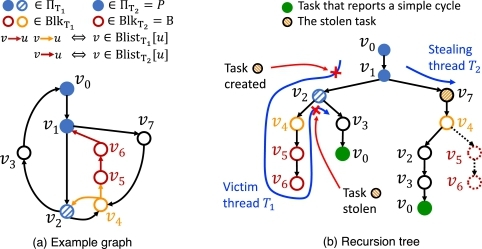
\includegraphics[width=0.7\textwidth]{images/figure-1.1.jpg}
  \caption{Περιγραφή πρώτης εικόνας πρώτου κεφαλαίου.}
  \label{fig:1.1}
\end{figure}

\subsubsection{Τίτλος \ldots}

\bigskip

\subsubsection{Τίτλος \ldots}

\bigskip

% Παράδειγμα: εικόνα εντός κειμένου
\begin{figure}[htbp]
  \centering
  
\includegraphics[width=0.5\textwidth]{images/figure-1.2.jpg}
  \caption{Περιγραφή δεύτερης εικόνας πρώτου κεφαλαίου.}
  \label{fig:1.2}
\end{figure}
